% !TEX root = main.tex
\documentclass[12pt,a4paper]{article}

\usepackage[T1]{fontenc}
\usepackage{graphicx}
\usepackage{titlesec}
\usepackage{setspace}
\usepackage{geometry}
\usepackage{array}
\usepackage{booktabs}
\usepackage{longtable}
\usepackage{amsmath}
\usepackage{amssymb}
\usepackage{mathptmx}
\usepackage{tikz}
\usepackage[colorlinks=true, linkcolor=blue, citecolor=blue, urlcolor=blue]{hyperref}
\usetikzlibrary{arrows.meta,positioning}

\geometry{
    left=30mm,
    right=25mm,
    top=25mm,
    bottom=25mm
}
\setstretch{1.15}
\setlength{\parindent}{0pt}
\titleformat{\section}{\large\bfseries}{\thesection.}{1em}{}
\titleformat{\subsection}{\normalsize\bfseries}{\thesubsection.}{1em}{}

\begin{document}
\hypersetup{pageanchor=false}

% --------- First Page (Cover Page) ---------
\begin{titlepage}
    \centering

    \vspace*{0.35cm}

    \begin{minipage}[t][0.86\textheight][s]{0.92\textwidth}
        \centering
        \vspace*{0.15cm}

        {\LARGE \textbf{University of Ruhuna}}\\[0.20cm]
        {\Large \textbf{Faculty of Engineering}}\\[0.15cm]
        \rule{0.78\textwidth}{0.8pt}

        \vfill

        {\Large \textbf{Take Home Assignment}}\\[0.40cm]
        {\huge \textbf{Assignment 1}}\\[0.20cm]
        \vfill

        {\Large \textbf{EE7220/EC7208}}\\[0.45cm]
        {\huge \textbf{Optimization Techniques for Engineers}}


        \vfill

        {\Large \textbf{Group Members}}\\[0.45cm]
        \renewcommand{\arraystretch}{1.3}
        \begin{tabular}{@{}>{\bfseries}p{0.14\textwidth}p{0.52\textwidth}p{0.24\textwidth}@{}}
            01 & Ashfaq M.R.M & EG/2021/4417 \\
            02 & Munsif M.F.A & EG/2021/4684 \\
        \end{tabular}
        \vspace*{0.15cm}
    \end{minipage}
    \vspace*{0.25cm}
\end{titlepage}
\hypersetup{pageanchor=true}
\renewcommand{\arraystretch}{1.15}

% --------- Assignment Content ---------
\section{HPC Cloud Server Resource Allocation (Knapsack Problem)}

\subsection{Scenario}
\textbf{LankaCloud Pvt Ltd} is a cloud computing provider based in Colombo, Sri Lanka. The company operates a
High-Performance Computing (HPC) server that can host managed application instances for its clients.
The server has a limited compute capacity shared among all hosted applications.

LankaCloud offers three types of managed application hosting packages:

\begin{center}
\begin{tabular}{c l c c}
\toprule
$k$ & Application Type & vCPU per instance & Monthly Profit per instance \\
\midrule
1 & Web Application Server & 3 vCPU & Rs. 7{,}000 \\
2 & Mobile API Server & 5 vCPU & Rs. 12{,}000 \\
3 & ML Inference Server & 9 vCPU & Rs. 25{,}000 \\
\bottomrule
\end{tabular}
\end{center}

The HPC server has a total capacity of \textbf{20 vCPU units}. Multiple instances of the same application
type may be hosted simultaneously. LankaCloud wants to determine how many instances of each application
type to host in order to \textbf{maximise total monthly profit}, subject to the server's capacity limit.

\subsection{Resource Abstraction: vCPU Unit}
Real HPC servers have multiple resource dimensions: CPU cores, RAM, and storage. To apply the standard
single-constraint Knapsack formulation, all resources are unified into a single \textbf{virtual CPU (vCPU)}
metric. Each vCPU unit represents a fixed bundle of:

\begin{itemize}
    \item 2 physical CPU cores
    \item 4 GB RAM
    \item 20 GB SSD storage
\end{itemize}

Total server capacity: 40 CPU cores / 80 GB RAM / 400 GB storage = \textbf{20 vCPU units}.

\subsection{Mathematical Formulation}
\textbf{Parameters:}
\begin{itemize}
    \item $N = 3$ (number of application types)
    \item $C = 20$ (total server capacity in vCPU units)
    \item $w_1 = 3,\; w_2 = 5,\; w_3 = 9$ (vCPU consumed per instance)
    \item $r_1 = 7{,}000,\; r_2 = 12{,}000,\; r_3 = 25{,}000$ (monthly profit in Rs. per instance)
\end{itemize}

\textbf{Decision Variables:}
\begin{itemize}
    \item $x_k$ = number of instances of application type $k$ to host (non-negative integer), $k=1,2,3$
\end{itemize}

\textbf{Objective Function:}
\[
\text{Maximise } Z = 7{,}000x_1 + 12{,}000x_2 + 25{,}000x_3
\]

\textbf{Capacity Constraint:}
\[
3x_1 + 5x_2 + 9x_3 \leq 20
\]

\textbf{Integrality Constraint:}
\[
x_1, x_2, x_3 \in \{0,1,2,\ldots\}
\]



\subsection{Dynamic Programming Formulation}

\textbf{Recurrence Relation:}
\[
V_k(i) = \max_{0 \le x_k \le i/w_k} \left[ r_k x_k + V_{k+1}(i - w_k x_k) \right]
\]

\subsection{Stage 3: ML Inference Server (w3 = 9, r3 = Rs. 25{,}000)}
\[
V_3(i)=\max_{0 \le x_3 \le i/9}\left[25{,}000\cdot x_3\right]
\]

\begin{center}
\begin{tabular}{c c c}
\toprule
Remaining Capacity ($i$) & Optimal $x_3^\ast$ & $V_3(i)$ (Rs.) \\
\midrule
0 & 0 & 0 \\
1 & 0 & 0 \\
2 & 0 & 0 \\
3 & 0 & 0 \\
4 & 0 & 0 \\
5 & 0 & 0 \\
6 & 0 & 0 \\
7 & 0 & 0 \\
8 & 0 & 0 \\
9 & 1 & 25{,}000 \\
10 & 1 & 25{,}000 \\
11 & 1 & 25{,}000 \\
12 & 1 & 25{,}000 \\
13 & 1 & 25{,}000 \\
14 & 1 & 25{,}000 \\
15 & 1 & 25{,}000 \\
16 & 1 & 25{,}000 \\
17 & 1 & 25{,}000 \\
18 & 2 & 50{,}000 \\
19 & 2 & 50{,}000 \\
20 & 2 & 50{,}000 \\
\bottomrule
\end{tabular}
\end{center}

\subsection{Stage 2: Mobile API Server + ML Inference (w2 = 5, r2 = Rs. 12{,}000)}
\[
V_2(i)=\max_{0 \le x_2 \le i/5}\left[12{,}000\cdot x_2 + V_3(i-5x_2)\right]
\]

\begin{center}
\resizebox{\textwidth}{!}{
\begin{tabular}{c c c c c c c c}
\toprule
$i$ &
$x_2{=}0: V_3(i)$ &
$x_2{=}1: 12k{+}V_3(i{-}5)$ &
$x_2{=}2: 24k{+}V_3(i{-}10)$ &
$x_2{=}3: 36k{+}V_3(i{-}15)$ &
$x_2{=}4: 48k{+}V_3(i{-}20)$ &
Optimal $x_2^\ast$ &
$V_2(i)$ (Rs.) \\
\midrule
0  & 0 & \textemdash & \textemdash & \textemdash & \textemdash & 0 & 0 \\
1  & 0 & \textemdash & \textemdash & \textemdash & \textemdash & 0 & 0 \\
2  & 0 & \textemdash & \textemdash & \textemdash & \textemdash & 0 & 0 \\
3  & 0 & \textemdash & \textemdash & \textemdash & \textemdash & 0 & 0 \\
4  & 0 & \textemdash & \textemdash & \textemdash & \textemdash & 0 & 0 \\
5  & 0 & 12{,}000 & \textemdash & \textemdash & \textemdash & 1 & 12{,}000 \\
6  & 0 & 12{,}000 & \textemdash & \textemdash & \textemdash & 1 & 12{,}000 \\
7  & 0 & 12{,}000 & \textemdash & \textemdash & \textemdash & 1 & 12{,}000 \\
8  & 0 & 12{,}000 & \textemdash & \textemdash & \textemdash & 1 & 12{,}000 \\
9  & 25{,}000 & 12{,}000 & \textemdash & \textemdash & \textemdash & 0 & 25{,}000 \\
10 & 25{,}000 & 12{,}000 & 24{,}000 & \textemdash & \textemdash & 0 & 25{,}000 \\
11 & 25{,}000 & 12{,}000 & 24{,}000 & \textemdash & \textemdash & 0 & 25{,}000 \\
12 & 25{,}000 & 12{,}000 & 24{,}000 & \textemdash & \textemdash & 0 & 25{,}000 \\
13 & 25{,}000 & 12{,}000 & 24{,}000 & \textemdash & \textemdash & 0 & 25{,}000 \\
14 & 25{,}000 & \textbf{37{,}000} & 24{,}000 & \textemdash & \textemdash & 1 & 37{,}000 \\
15 & 25{,}000 & \textbf{37{,}000} & 24{,}000 & 36{,}000 & \textemdash & 1 & 37{,}000 \\
16 & 25{,}000 & \textbf{37{,}000} & 24{,}000 & 36{,}000 & \textemdash & 1 & 37{,}000 \\
17 & 25{,}000 & \textbf{37{,}000} & 24{,}000 & 36{,}000 & \textemdash & 1 & 37{,}000 \\
18 & \textbf{50{,}000} & 37{,}000 & 24{,}000 & 36{,}000 & \textemdash & 0 & 50{,}000 \\
19 & \textbf{50{,}000} & 37{,}000 & 49{,}000 & 36{,}000 & \textemdash & 0 & 50{,}000 \\
20 & \textbf{50{,}000} & 37{,}000 & 49{,}000 & 36{,}000 & 48{,}000 & 0 & 50{,}000 \\
\bottomrule
\end{tabular}
}
\end{center}


\subsection{Stage 1: All Application Types (Capacity = 20 vCPU)}
\[
V_1(20)=\max_{0 \le x_1 \le 20/3}\left[7{,}000\cdot x_1 + V_2(20-3x_1)\right]
\]

\begin{center}
\resizebox{\textwidth}{!}{
\begin{tabular}{c c c c c}
\toprule
$x_1$ & $7{,}000\times x_1$ (Rs.) & Remaining capacity $(20-3x_1)$ & $V_2(20-3x_1)$ (Rs.) & Total (Rs.) \\
\midrule
0 & 0 & 20 & 50{,}000 & 50{,}000 \\
1 & 7{,}000 & 17 & 37{,}000 & 44{,}000 \\
\textbf{2} & \textbf{14{,}000} & \textbf{14} & \textbf{37{,}000} & \textbf{51{,}000} \\
3 & 21{,}000 & 11 & 25{,}000 & 46{,}000 \\
4 & 28{,}000 & 8 & 12{,}000 & 40{,}000 \\
5 & 35{,}000 & 5 & 12{,}000 & 47{,}000 \\
6 & 42{,}000 & 2 & 0 & 42{,}000 \\
\bottomrule
\end{tabular}
}
\end{center}

\textbf{Optimal decision at Stage 1:} $x_1^\ast = 2$

\subsection{Traceback: Recovering the Optimal Solution}
\begin{center}
\begin{tabular}{c c c c c c}
\toprule
Step & Stage & Remaining capacity & Optimal $x_k^\ast$ & vCPU used & Profit earned \\
\midrule
1 & $k=1$ & 20 & $x_1^\ast=\textbf{2}$ & $2\times3=6$ & $2\times7{,}000=\text{Rs. }14{,}000$ \\
2 & $k=2$ & $20-6=14$ & $x_2^\ast=\textbf{1}$ & $1\times5=5$ & $1\times12{,}000=\text{Rs. }12{,}000$ \\
3 & $k=3$ & $14-5=9$ & $x_3^\ast=\textbf{1}$ & $1\times9=9$ & $1\times25{,}000=\text{Rs. }25{,}000$ \\
\bottomrule
\end{tabular}
\end{center}

\textbf{Total vCPU used:} $6+5+9 = \textbf{20/20}$ (server fully utilised)

\subsection{Optimal Solution}
\begin{quote}
Host
2 Web Application Servers, 
1 Mobile API Server, and 
1 ML Inference Server.

Maximum monthly profit = Rs. 14{,}000 + Rs. 12{,}000 + Rs. 25{,}000 = Rs. 51{,}000
\end{quote}

\subsection{Why Greedy Fails}
A greedy approach ranks applications by profit-per-vCPU (value-to-weight ratio):

\begin{center}
\begin{tabular}{l c c}
\toprule
Application Type & Profit/vCPU & Greedy rank \\
\midrule
ML Inference Server & $25{,}000/9 \approx \textbf{2{,}778}$ & 1st \\
Mobile API Server & $12{,}000/5 = \textbf{2{,}400}$ & 2nd \\
Web Application & $7{,}000/3 \approx \textbf{2{,}333}$ & 3rd \\
\bottomrule
\end{tabular}
\end{center}

\textbf{Greedy execution (capacity = 20 vCPU):}
\begin{enumerate}
    \item Pick ML Inference (9 vCPU) $\rightarrow$ capacity remaining: 11 vCPU, profit: Rs. 25{,}000
    \item Pick ML Inference again (9 vCPU) $\rightarrow$ capacity remaining: 2 vCPU, profit: Rs. 50{,}000
    \item No application fits in 2 vCPU $\rightarrow$ \textbf{stop}
\end{enumerate}

\textbf{Greedy result:} $x_1=0,\; x_2=0,\; x_3=2 \rightarrow \textbf{Rs. 50{,}000}$ (2 vCPU wasted)

\begin{center}
\begin{tabular}{l c c c c c}
\toprule
Method & $x_1$ & $x_2$ & $x_3$ & vCPU used & Monthly Profit \\
\midrule
Greedy & 0 & 0 & 2 & $18/20$ & Rs. 50{,}000 \\
\textbf{DP} & \textbf{2} & \textbf{1} & \textbf{1} & \textbf{20/20} & \textbf{Rs. 51{,}000} \\
\bottomrule
\end{tabular}
\end{center}

So greedy wastes 2 vCPU and earns Rs. 1{,}000 less per month. The DP approach avoids this by checking
every feasible combination at each stage, so no capacity goes unused unnecessarily.

\section{Network Optimization Using the Reverse-Delete MST Algorithm}
\subsection{Emergency Fiber Network for Disaster Response}

A city needs to connect 10 critical facilities with a fiber communication network that can hold
up during floods and cyclones. Engineers have surveyed several possible cable routes along
existing roads. The goal is to make sure all facilities can reach each other (directly or via
other nodes) while keeping total installation cost as low as possible.

\subsection{Graph Model}
\subsubsection{Facilities (Vertices)}
\begin{itemize}
    \item H: Main Hospital
    \item P: Police HQ
    \item F: Fire Station
    \item G: City Hall / Disaster Control Center
    \item W: Water Treatment Plant
    \item U: Power Substation
    \item T: Telecom Hub
    \item S: Central School (relief center)
    \item M: Main Market (supplies hub)
    \item B: Bus Depot (evacuation transport)
\end{itemize}

\subsubsection{Candidate Fiber Links (Edges with Costs)}
Costs are expressed in generic installation cost units. The network is undirected.

\begin{center}
\begin{tabular}{c c c c}
\toprule
Edge & Cost & Edge & Cost \\
\midrule
H-G & 22 & M-B & 21 \\
T-B & 20 & U-B & 19 \\
W-B & 18 & W-U & 17 \\
S-M & 16 & G-T & 15 \\
G-S & 14 & F-B & 13 \\
F-G & 12 & P-M & 11 \\
P-G & 10 & H-T & 9 \\
H-P & 8 & H-F & 7 \\
H-S & 6 & P-F & 5 \\
G-U & 4 & S-W & 3 \\
U-T & 2 & T-M & 1 \\
\bottomrule
\end{tabular}
\end{center}

This is essentially a Minimum Spanning Tree (MST) problem — we want the cheapest set of links
that still keeps all 10 facilities connected. With 10 nodes, the spanning tree will always have
exactly 9 edges.

\subsection{Selected MST Technique: Reverse-Delete Algorithm}

For a connected, undirected, weighted graph $G=(V,E)$, an MST is a subset of edges $T\subseteq E$ that
connects all vertices, contains no cycles, and minimizes total weight $\sum_{e \in T} w(e)$.

The Reverse-Delete algorithm works on the cycle property: within any cycle in the graph, the heaviest
edge is not needed for the MST. Removing it still leaves every vertex reachable through the remaining
edges in the cycle, just at a lower cost.

\subsubsection{Steps}
\begin{enumerate}
    \item Take the full graph with all candidate links.
    \item Sort all edges from highest cost to lowest.
    \item Go through each edge: try removing it. If the network is still connected, drop it for good.
    If removing it disconnects anything, put it back and move on.
    \item Whatever edges remain at the end form the MST.
\end{enumerate}

This approach suits the scenario well — the city already has a full list of proposed cable routes,
and the algorithm trims the expensive ones first without ever breaking connectivity.

\subsection{Step-by-Step Application of Reverse-Delete}
\subsubsection{Edge Order (Descending)}
Edges are processed from highest cost to lowest cost:
22, 21, 20, 19, 18, 17, 16, 15, 14, 13, 12, 11, 10, 9, 8, 7, 6, 5, 4, 3, 2, 1.

\subsubsection{Reverse-Delete Decision Table}
Each edge is checked in order — if removing it keeps the graph connected it gets deleted, otherwise it stays.

\begingroup
\small
\setlength{\tabcolsep}{3pt}
\begin{longtable}{c c c c p{8.5cm}}
\toprule
Step & Edge & Cost & Decision & Connectivity check (reason) \\
\midrule
\endfirsthead
\toprule
Step & Edge & Cost & Decision & Connectivity check (reason) \\
\midrule
\endhead
\bottomrule
\endfoot
1 & H-G & 22 & REMOVE & H still reaches G via H-T-U-G. \\
2 & M-B & 21 & REMOVE & M still reaches B via M-T-B (later replaced by M-T-U-B paths; at this step B-links still exist). \\
3 & T-B & 20 & REMOVE & T still reaches B via T-U-B. \\
4 & U-B & 19 & REMOVE & U still reaches B via U-W-B. \\
5 & W-B & 18 & REMOVE & W still reaches B via W-U-G-F-B. \\
6 & W-U & 17 & REMOVE & W still reaches U via W-S-H-T-U. \\
7 & S-M & 16 & REMOVE & S still reaches M via S-H-T-M. \\
8 & G-T & 15 & REMOVE & G still reaches T via G-U-T. \\
9 & G-S & 14 & REMOVE & G still reaches S via G-U-T-H-S. \\
10 & F-B & 13 & KEEP & If removed, B becomes isolated (all other B links have already been deleted). \\
11 & F-G & 12 & REMOVE & F still reaches G via F-H-T-U-G. \\
12 & P-M & 11 & REMOVE & P still reaches M via P-F-H-T-M. \\
13 & P-G & 10 & REMOVE & P still reaches G via P-F-H-T-U-G. \\
14 & H-T & 9 & KEEP & If removed, the graph splits \{G,U,T,M\} from \{H,S,W,F,P,B\}. \\
15 & H-P & 8 & REMOVE & H still reaches P via H-F-P. \\
16 & H-F & 7 & KEEP & If removed, \{F,P,B\} disconnects from the rest. \\
17 & H-S & 6 & KEEP & If removed, \{S,W\} disconnects (S has no other remaining links). \\
18 & P-F & 5 & KEEP & If removed, P becomes isolated (H-P already deleted). \\
19 & G-U & 4 & KEEP & If removed, G becomes isolated (all other G links were deleted). \\
20 & S-W & 3 & KEEP & If removed, W becomes isolated (W-U and W-B were deleted). \\
21 & U-T & 2 & KEEP & If removed, \{U,G\} disconnects from the rest. \\
22 & T-M & 1 & KEEP & If removed, M becomes isolated (S-M and P-M were deleted). \\
\end{longtable}
\endgroup

\subsection{Final MST and Minimum Total Cost}
After processing all edges, the remaining edges (marked KEEP) form the MST.

\begin{center}
\begin{tabular}{c c}
\toprule
MST edge & Cost \\
\midrule
T-M & 1 \\
U-T & 2 \\
S-W & 3 \\
G-U & 4 \\
P-F & 5 \\
H-S & 6 \\
H-F & 7 \\
H-T & 9 \\
F-B & 13 \\
\bottomrule
\end{tabular}
\end{center}

Total minimum cost $= 1 + 2 + 3 + 4 + 5 + 6 + 7 + 9 + 13 = 50$.

One way to visualize the final tree (connectivity path) is:

W - S - H - T - U - G, with branches H - F - P and F - B, and T - M.

\subsection{Graph Overview}
The graphs below provide a visual summary of the Reverse-Delete decisions and the final MST structure.

\textbf{Remove vs Keep Decisions:}
\begin{center}
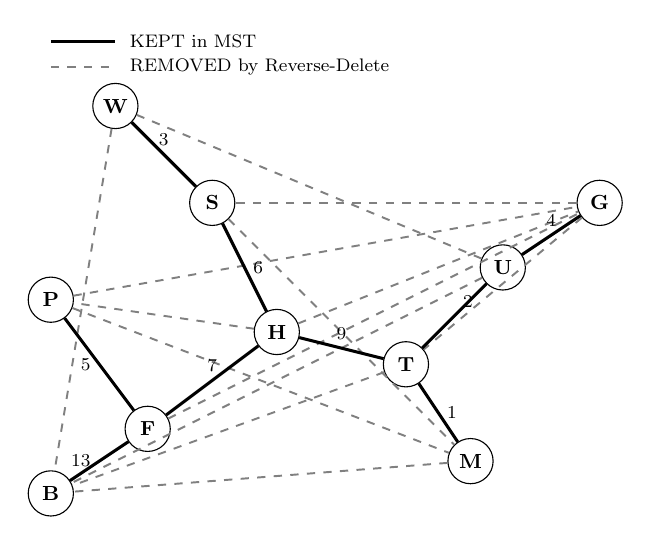
\begin{tikzpicture}[
    scale=0.82,
    transform shape,
    facility/.style={circle,draw,minimum size=7mm,inner sep=0pt,font=\small\bfseries,fill=white},
    kept/.style={line width=1.1pt},
    removed/.style={draw=gray,dashed,line width=0.7pt}
]
    % Node layout follows MST tree: H is central hub
    \node[facility] (H) at (0, 0)    {H};
    \node[facility] (S) at (-1, 2)   {S};
    \node[facility] (W) at (-2.5,3.5){W};
    \node[facility] (F) at (-2,-1.5) {F};
    \node[facility] (P) at (-3.5,0.5){P};
    \node[facility] (B) at (-3.5,-2.5){B};
    \node[facility] (T) at (2,-0.5)  {T};
    \node[facility] (M) at (3,-2)    {M};
    \node[facility] (U) at (3.5,1)   {U};
    \node[facility] (G) at (5,2)     {G};

    % Removed edges (dashed gray)
    \draw[removed] (H) -- (G);
    \draw[removed] (M) -- (B);
    \draw[removed] (T) -- (B);
    \draw[removed] (U) -- (B);
    \draw[removed] (W) -- (B);
    \draw[removed] (W) -- (U);
    \draw[removed] (S) -- (M);
    \draw[removed] (G) -- (T);
    \draw[removed] (G) -- (S);
    \draw[removed] (F) -- (G);
    \draw[removed] (P) -- (M);
    \draw[removed] (P) -- (G);
    \draw[removed] (H) -- (P);

    % Kept edges (MST)
    \draw[kept] (T) -- node[right]      {\footnotesize 1} (M);
    \draw[kept] (U) -- node[above right]{\footnotesize 2} (T);
    \draw[kept] (S) -- node[above]      {\footnotesize 3} (W);
    \draw[kept] (G) -- node[above]      {\footnotesize 4} (U);
    \draw[kept] (P) -- node[left]       {\footnotesize 5} (F);
    \draw[kept] (H) -- node[right]      {\footnotesize 6} (S);
    \draw[kept] (H) -- node[above]      {\footnotesize 7} (F);
    \draw[kept] (H) -- node[above]      {\footnotesize 9} (T);
    \draw[kept] (F) -- node[left]       {\footnotesize 13}(B);

    % Legend (top-left, above W)
    \draw[kept] (-3.5,4.5) -- (-2.5,4.5);
    \node[anchor=west,font=\footnotesize] at (-2.4,4.5) {KEPT in MST};
    \draw[removed] (-3.5,4.1) -- (-2.5,4.1);
    \node[anchor=west,font=\footnotesize] at (-2.4,4.1) {REMOVED by Reverse-Delete};
\end{tikzpicture}
\end{center}

Dashed links were removed because the network stayed connected without them. Solid links
are the ones that had to be kept — removing any of them would have split the network.
These 9 solid links form the final MST with total cost 50.

\textbf{Final MST (selected links only):}
\begin{center}
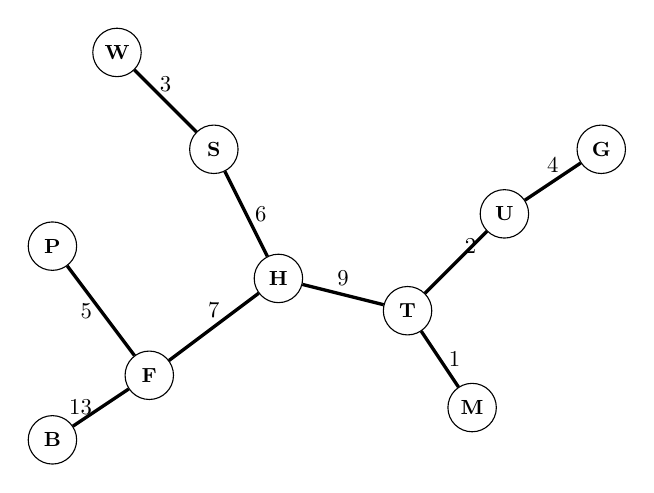
\begin{tikzpicture}[
    scale=0.82,
    transform shape,
    facility/.style={circle,draw,minimum size=7.5mm,inner sep=0pt,font=\small\bfseries,fill=white},
    mst/.style={line width=1.2pt}
]
    % Same layout as the Remove/Keep graph above
    \node[facility] (H) at (0, 0)    {H};
    \node[facility] (S) at (-1, 2)   {S};
    \node[facility] (W) at (-2.5,3.5){W};
    \node[facility] (F) at (-2,-1.5) {F};
    \node[facility] (P) at (-3.5,0.5){P};
    \node[facility] (B) at (-3.5,-2.5){B};
    \node[facility] (T) at (2,-0.5)  {T};
    \node[facility] (M) at (3,-2)    {M};
    \node[facility] (U) at (3.5,1)   {U};
    \node[facility] (G) at (5,2)     {G};

    \draw[mst] (T) -- node[right]      {1}  (M);
    \draw[mst] (U) -- node[above right]{2}  (T);
    \draw[mst] (S) -- node[above]      {3}  (W);
    \draw[mst] (G) -- node[above]      {4}  (U);
    \draw[mst] (P) -- node[left]       {5}  (F);
    \draw[mst] (H) -- node[right]      {6}  (S);
    \draw[mst] (H) -- node[above]      {7}  (F);
    \draw[mst] (H) -- node[above]      {9}  (T);
    \draw[mst] (F) -- node[left]       {13} (B);
\end{tikzpicture}
\end{center}

\textbf{MST cost from the graph:} $1+2+3+4+5+6+7+9+13=50$.

\end{document}
